\chapter{Conclusions and results}
\label{ch:results}

Aurora succesfuly estimates direct illumination in arbitrary scenes via stochastic Monte Carlo raytracing. Achieved performance is promising althorugh not yet adequate for interactive rendering. Autodesk Maya integration makes it a robust and easy to use tool for offline 3D scene visualisation.

\section{Further work}
There is a significant amount of possible future improvements in Aurora.
\begin{itemize}
\item Right now only direct illumination is estimated. Addition of a global illumination algorithm would greatly increase realism by also estimating indirect illumination due to phenomena like diffuse interreflection.
\item Adding support for more complex BRDFs, for example micorfacet models or anisotropic distributions, would be also beneficial to rendering realism.
\item Extending sampling strategies to pseudo Monte Carlo sampling, for example by employing Halton sequences or stratified sampling, would reduce variance and produce images with less noise.
\item Adding multiple GPU support would greatly increase performance on systems with more than one CUDA capable graphics card.
\end{itemize}
\vfill

\section{Example renders}
All images showed in this section were produced with Aurora in Autodesk Maya 2014 on 64--bit Windows 7 system. 

Rendering was performed on a PC equipped with Intel Core i5-3470 processor, 16 GB of RAM and a single NVIDIA GTX 560 Ti graphics card with 1GB of dedicated on--board video memory.

The 3D scene is \emph{Crytek Sponza Atrium}\footnote{\url{http://www.crytek.com/cryengine/cryengine3/downloads}} by Frank Meinl, a widely used test scene for evaluating the performance of rendering algorithms.

Geometry for this scene consists of more than 262,000 triangles. The NMH build time was 1.7 seconds. The images were rendered in full HD 1920x1080 resolution taking 4 image samples per pixel.

\begin{figure}[htb]
  \begin{center}
    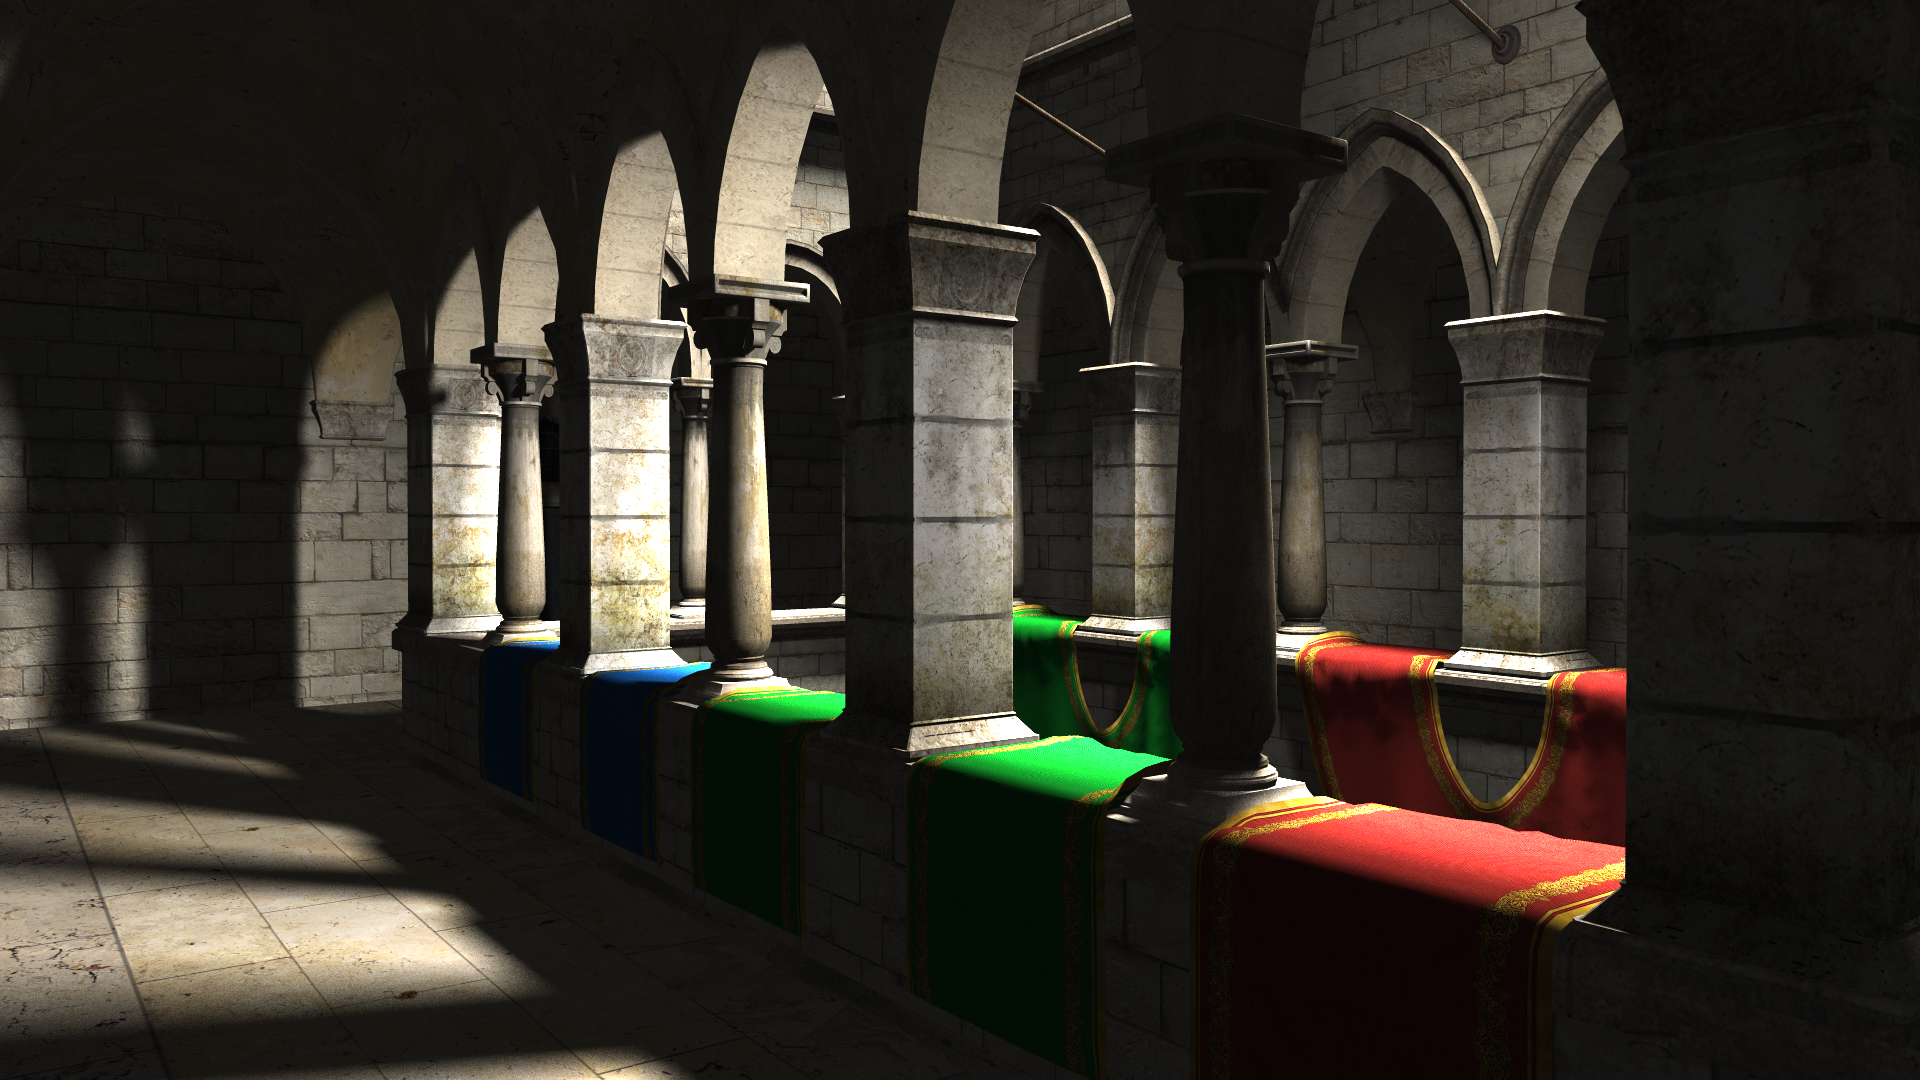
\includegraphics[width=\textwidth]{chapters/results/sponza_softshadows.png}
  \end{center}
  \caption{Test scene illuminated by 3 area lights, with 64 shadow samples per light. Rendering time was about 7 minutes.}
\end{figure}

\begin{figure}[htb]
  \begin{center}
    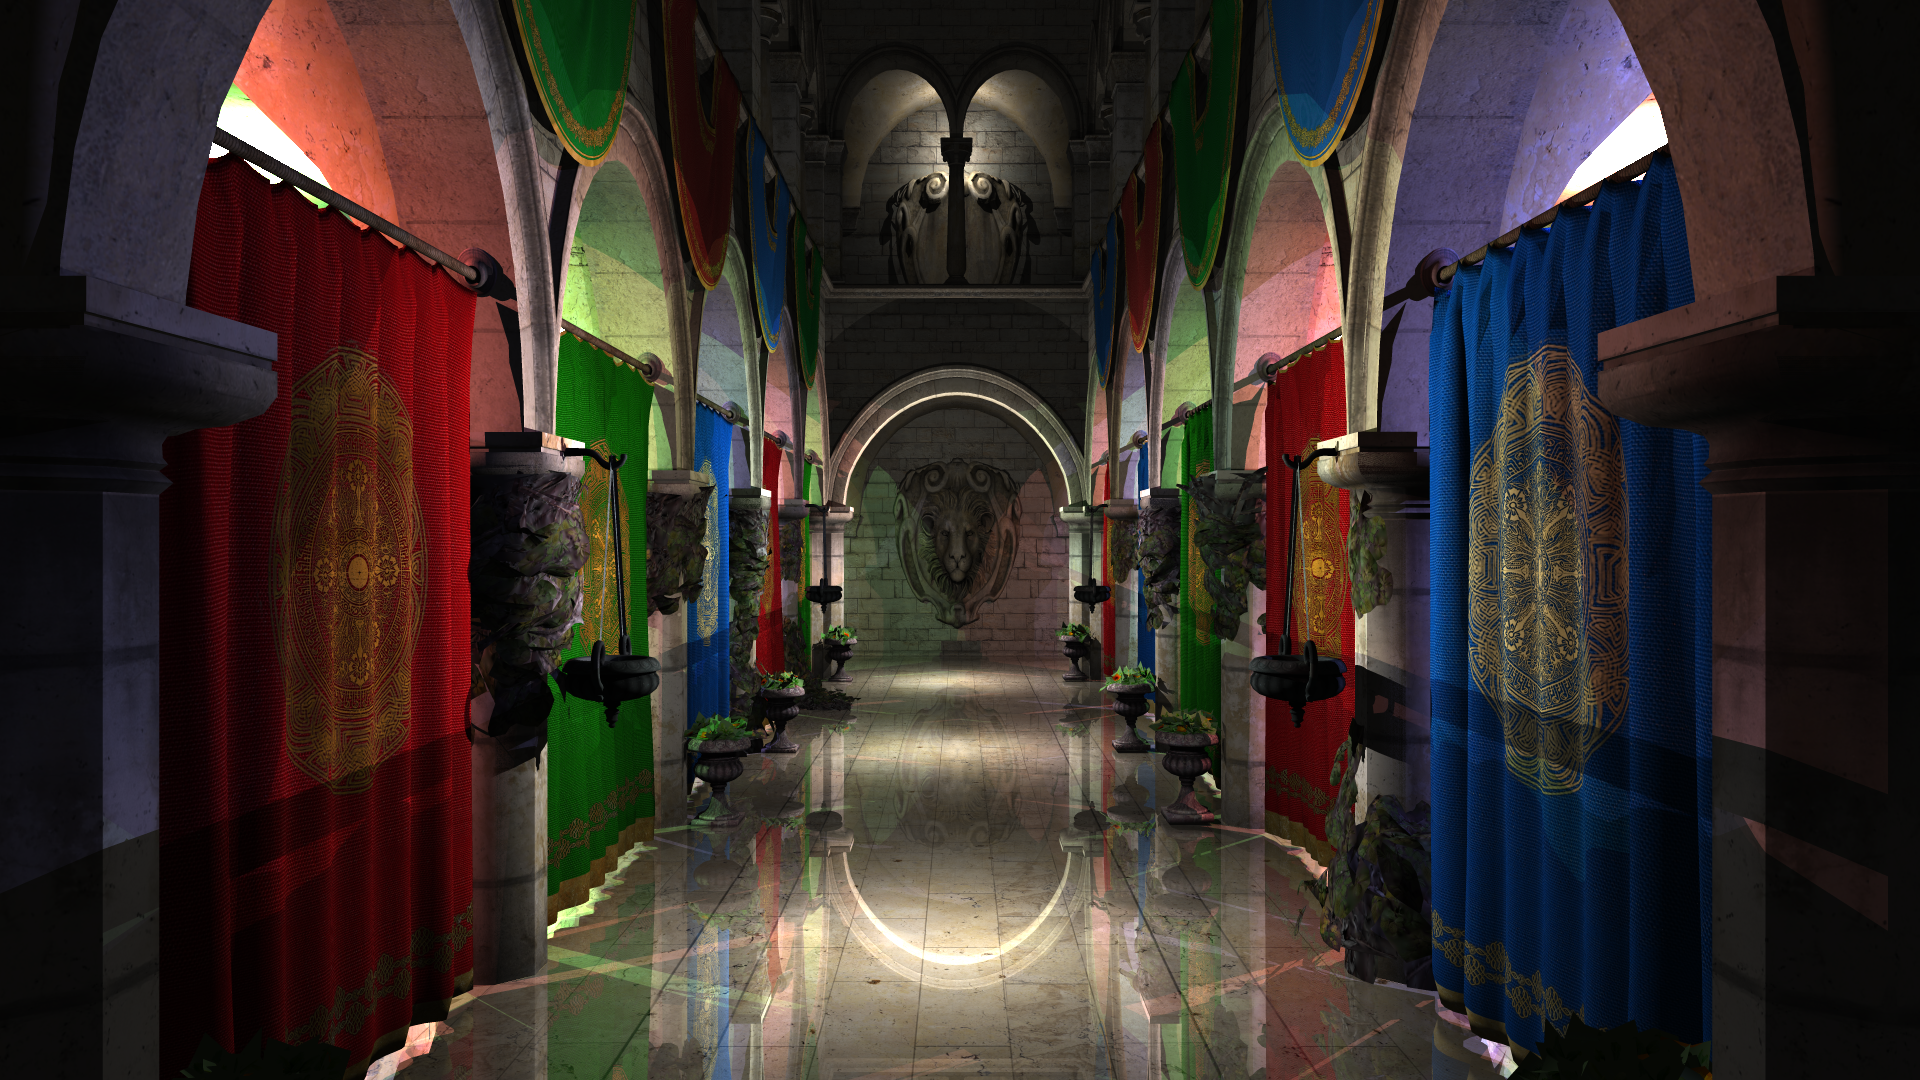
\includegraphics[width=\textwidth]{chapters/results/sponza_manypoint.png}
  \end{center}
  \caption{Test scene illuminated by 14 point lights. Rendering time was about 2.5 minutes.}
\end{figure}

\begin{figure}[htb]
  \begin{center}
    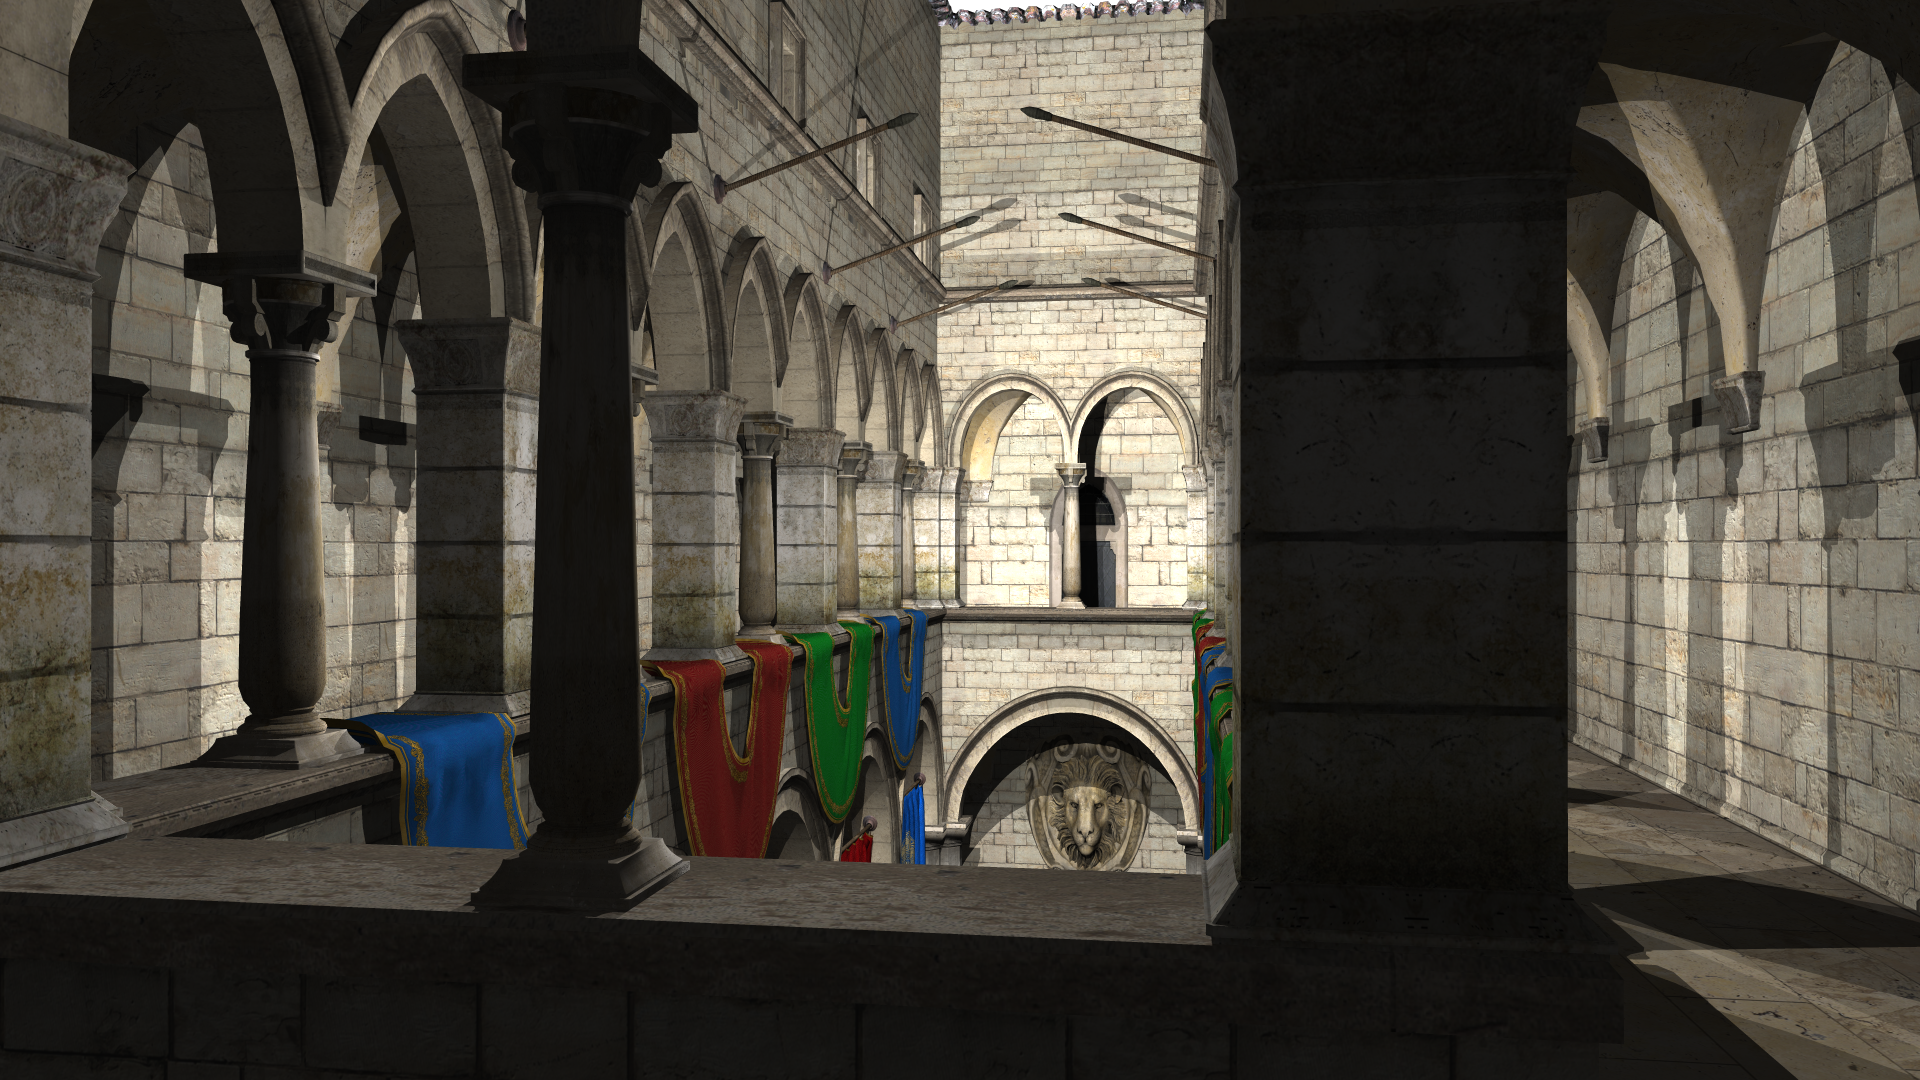
\includegraphics[width=\textwidth]{chapters/results/sponza_point.png}
  \end{center}
  \caption{Test scene illuminated by 3 point lights with no distance falloff. Rendering time was about 18 seconds.}
\end{figure}
